
\documentclass[draft=true, 12pt]{report}
\input{bayesuvius.sty}
\begin{document}

\subsection{Frobenius Theorem}

One common problem 
in Differential Geometry is: suppose you are given a surface (or, more generally, a manifold),
find its tangent planes. Frobenius Theorem addresses the reverse question:
suppose you are given a 
family of planes, do they 
determine a surface (or manifold). 

As an example of case
where a family
of planes
fails to determine a surface,
consider the following 1-form

\beq
\pform{\omega}{}=
x\ul{dy} + \ul{dz}
\label{eq-shear-dif-form1}
\eeq
$\ul{\omega}=0$ means
you have 1 equation and 3 unknowns  $(dx, dy, dx)$.
So it is plausible 
that the 2 remaining degrees of freedom  determine a continuous 2-dim 
surface:

\beq
f(x, y, z)=0
\eeq
If that were the case, we 
would say that $\ul{\omega}=0$
is an {\bf integrable system
of equations}.
However, that is not the case 
here,
as can be seen from Fig.\ref{fig-stadard_contact_structure}

\begin{figure}[h!]
\centering
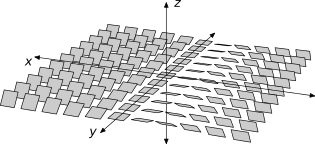
\includegraphics[width=3in]
{differ-geo/standard_contact_structure.png}
\caption{Dif-form $\ul{\omega}= x\ul{dy}+ \ul{dz}$ generates the
family of planes
shown. 
This family of planes fails to determine a surface. Indeed, if you tried to lay a rug on this figure, its $z$ coordinate would decrease with each right-handed turn about the $+Z$ axis.
Notice that the family of planes seems to turn around a  \qt{vortex}, the $Z$ axis.
It has \qt{vorticity}.
(This figure comes from the Wikipedia article for \qt{Frobenius theorem}. I changed the $X$ and $Y$
axes to fit my example.)}
\label{fig-stadard_contact_structure}
\end{figure}
In Fig.\ref{fig-stadard_contact_structure},
a family of planes fails to
determine a surface; i.e., it's not possible to lay a 
continuous rug over the
family of planes. 
When the opposite is the case
and it is possible to lay a rug, then one can lay multiple rugs, stacked one  on 
top of the other. Whenever
this is  possible, we say it
is possible to {\bf foliate} the manifold.
So integrability and 
foliability
are the same thing.
Both are global properties
of a manifold.

Frobenius Theorem (FT)
is a theorem
about one or more 1-forms. 
{\bf Contact Geometry} (see
Section \ref{sec-contact-geo})
studies 1-forms that
violate Frobenius Theorem
maximally.

\hrule
Simple Example from Fluid Mechanics

Consider the velocity field $\vecv =[\ul{\omega}]^\sharp$ 
for  the 1-form $\ul{\omega}$
given by Eq.(\ref{eq-shear-dif-form1}).

\beq
\vecv = x \hat{y} + a\hat{z}
\eeq

\beq
\nabla \times \vecv = 
\left|
\begin{array}{ccc}
\hat{x} &\hat{y}&\hat{z}
\\
\partial_1 &\partial_2 &\partial_3
\\
0 & x & a
\end{array}
\right|
= \hat{z}
\eeq

\beq
\vecv\cdot (\nabla \times \vecv)= 
\hat{z}\cdot [x \hat{y} +a \hat{z}] = a
\eeq

For a  fluid, $\nabla \times \vecv$ is called
the {\bf vorticity} and 
$\vecv \cdot (\nabla\times \vecv)$
is called the
{\bf helicity density}. 
Flows with non-zero helicity density
can occur in Nature and be solutions
of Navier-Stokes equation.
No viscosity or turbulence
is required to have them.

Note that when $a=0$, $\nabla \times \vecv$ is still the same,
but $\vecv\cdot (\nabla \times \vecv)=0$. 
That's because 
non-zero 
$\vecv\cdot (\nabla \times \vecv)$ is impossible to achieve in 2-dim.

\begin{figure}[h!]
\centering
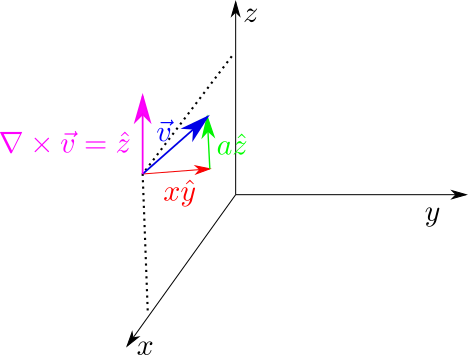
\includegraphics[width=3in]
{differ-geo/helicity-example.png}
\caption{Velocity field $\vecv = x \hat{y} + a\hat{z}$ has vorticity and
helicity density.}
\label{fig-helicity-example}
\end{figure}



A velocity field is said to be 
{\bf integrable}  if
and only if its streamlines
at every   point $\pi$ 
fall on a plane. 
For non-integrable velocity fields,
if you create a plane at a point $\pi$ with a bunch of streamlines,
then there will
exist other streamlines at $\pi$
that exit the plane.
Frobenius' Theorem for 
3-dim fluid flows is the statement
that a velocity field is integrable
iff it has zero helicity  density everywhere.
\hrule
Fluid Mechanics, in general

In general

\beq
\vecv\cdot(\nabla \times \vecv)= v_1(\partial_2 v_3 -\partial_3v_2)
+ \cpermu{123}
\eeq
If $\vecv$ is 2-dim, then we can rotate it so that $v_3=\partial_3=0$. Hence, 
the helicity  is zero.

\begin{claim}

\beq
\nabla\times (\lam \nabla f)=
\nabla \lam \times \nabla f
\eeq


\end{claim}
\proof

\beqa
\nabla\times (\lam f)=&=&
\left|
\begin{array}{ccc}
\hat{x}& \hat{y}&\hat{z}
\\
\partial_1
&\partial_2
 &\partial_3
\\
\lam \partial_1f
&\lam \partial_2f
&\lam \partial_3 f
\end{array}
\right|
\\
&=&
\left|
\begin{array}{ccc}
\hat{x}& \hat{y}&\hat{z}
\\
\partial_1 \lam 
&\partial_2 \lam  
&\partial_3 \lam 
\\
\partial_1f
&\partial_2f
&\partial_3 f
\end{array}
\right|
\eeqa
\qed

\begin{claim} 
$\vecv$ has zero helicity 
density iff there
exist functions 
$\lam(\vecr)$ and $f(\vecr)$
such that
$\vecv=\lam \nabla f$ 
\end{claim}
\proof

proof of $\revimplies$

\beqa
\vecv\cdot (\nabla \times \vecv)
&=&
\lam\nabla f\cdot
(\nabla \times (\lam\nabla f))
\\
&=&
\lam\nabla f
\cdot (\nabla \lam \times \nabla f)
\\
&=&
\lam
\left|
\begin{array}{ccc}
\partial_1 f
&\partial_2 f
&\partial_3 f
\\
\partial_1 \lam
&\partial_2 \lam
&\partial_3 \lam
\\
\partial_1 f
&\partial_2 f
&\partial_3 f
\end{array}
\right|
\\
&=&
0
\eeqa

\qed

Notice that 

\beq
\vecv =\lam \nabla f
\iff 
\ul{\omega}= [\vecv]^\flat=
\lam [\nabla f]^\flat= \lam \ul{df}
\eeq
Whether you think
of it in terms of 
vector calculus or  1-forms,
the meaning is the same.
Both $\vecv$ and $\nabla f$
point in the same
direction,
perpendicular to contour surfaces. But the factor 
of $\lam$ adjusts locally
the separation between
the contour surfaces. A special
\qt{rug thickness}
adjustment
causes $\vecv$ to
have zero helicity density.

\begin{claim}
Suppose

\beq
\ul{\omega} = v_1 \ul{dx} + v_2 \ul{dy}
+ v_3 \ul{dz}
=
(\vecv)^\flat
\eeq
Then

\beq 
\ul{\omega}\wedge d\ul{\omega}=
0
\quad
\text{iff}\quad
\vecv\cdot (\nabla \times \vecv)=0
\eeq
\end{claim}
\proof

\beq 
d\ul{\omega}=
(\partial_2 v_3 -\partial_3 v_2)
\ul{dy}\wedge \ul{dz} + \cpermu{123}
\eeq

\beqa
\ul{\omega}\wedge
d\ul{\omega} &=&
v_1 (\partial_2 v_3 -\partial_3 v_2)
\ul{dx}\wedge \ul{dy}\wedge \ul{dz}
+ \cpermu{123}
\\
&=&
\vecv\cdot(\nabla \times \vecv)
\ul{dx}\wedge \ul{dy}\wedge \ul{dz}
\eeqa

\qed

\hrule
Frobenius Theorem for single
1-form  and family of 1-forms

Frobenius Theorem (FT)
is a theorem
about one or more 1-forms. 
We first state FT
for a single 1-form.
Then we generalize FT to
a family of 1-forms.

\begin{claim}(Frobenius 
Theorem
for single 1-form)

Suppose $\pform{\omega}{}$
is a smooth 1-form in
an $n$ dimensional
manifold $M$.
Suppose

\beq
\ul{\omega}(\vecX)=0
\eeq
for all vector fields $\vecX$.
Define the {\bf distribution}

\beq
\cald_\pi = \{\vecX\in T_\pi(M):
\ul{\omega}(\vecX)=0\}
\eeq
Then the following statements 
are equivalent
\begin{enumerate}[(a)]
\item $\cald_\pi$ 
determines a continuous  $n-1$ dimensional hypersurface.
$\cald_\pi$ is said to bee {\bf integrable}.



\item There exist functions $\lam(\vecX)$ and $f(\vecX)$ such that

\beq
\ul{\omega}(\vecX)=
\lam(\vecX)\ul{df(\vecX)}
\eeq

\item $\pform{\omega}{}$ satisfies  

\beq
\pform{\omega}{}\wedge
d\pform{\omega}{}=0
\eeq
(always satisfied for $n\leq 2$)

\item For any $\vecX, \vecY \in \Gamma(\cald)$



\beq
[\vecX, \vecY]\in \cald
\eeq 
This is called {\bf involutivity}.
Here $\Gamma(\cald)$ are all the
vectors tangent to $\cald$.
The difference between
$\cald_\pi$, $\cald$ and 
$\Gamma(\cald)$ 
is discussed in Section 
\ref{sec-diff-f-fb-fs}.






\end{enumerate}
\end{claim}
\proof
\qed


\begin{claim}(Frobenius 
Theorem
for family of independent 1-forms)

Suppose $\{\pform{\omega^\alp}{}\}_{\alp=1}^A$
is a family of $A$ INDEPENDENT  smooth 1-forms in
an $n$ dimensional
manifold $M$.
Suppose

\beq
\ul{\omega^\alp}(\vecX)=0, \quad \text{for } \alp=1, 2, \ldots A
\eeq
for all vector fields $\vecX$.
Define the {\bf distribution}


\beq
\cald_\pi = \{\vecX\in T_\pi(M):
\ul{\omega^\alp}(\vecX)=0 \text{ for }\alp=1, 2, \ldots A\}
\eeq
Then the following statements 
are equivalent
\begin{enumerate}[(a)]
\item $\cald_\pi$ 
determines a continuous  $A-1$ dimensional hypersurface.
$\cald_\pi$ is said to be {\bf integrable}.

\item There exist 
1-forms $\{\pform{\lam\indices{^\alp_\beta}}{}\}$
such that  
\beq
\pform{d\omega^\alp}
{2}=
\sum_\beta
\pform{\lam\indices{^\alp_\beta}}{}
\wedge
\pform{\omega^\beta}{}
\eeq
This statement can be phrased in terms of 
dif-form ideals. Dif-form ideals
are discussed in Section 
\ref{sec-dif-form-ideal}.

\item For any $\vecX, \vecY \in \Gamma(\cald)$



\beq
[\vecX, \vecY]\in \cald
\eeq 
This is called {\bf involutivity}.
Here $\Gamma(\cald)$ are all
vectors tangent to $\cald$.
The difference between
$\cald_\pi$, $\cald$ and 
$\Gamma(\cald)$ 
is discussed in Section 
\ref{sec-diff-f-fb-fs}.
\end{enumerate}

\end{claim}
\proof

Note that for a single 
1-form, 

\beq
\ul{d\omega}=\ul{\lam}\wedge \ul{\omega}
\implies
\ul{\omega}\wedge \ul{d\omega}=
\ul{\omega}
\wedge
(\ul{\lam}\wedge \ul{\omega})
=0
\eeq
\qed
\subsubsection{Dif-form Ideals}
\label{sec-dif-form-ideal}

A {\bf dif-form (PF) ideal} $\cali$ is a set
of dif-forms that satisfies the following condition:

\begin{enumerate}
\item $\ul{\alp}\in \cali$ implies 
$\ul{\alp}\wedge \ul{\beta}\in \cali$ for any dif-form $
\ul{\beta}$ of any degree.
\end{enumerate}

Ideals are often specified by giving
a set of generators. 
Then the ideal is the set
of all dif-forms that have the generators as
\qt{factors} under the wedge product.
For example, 
the ideal with
generators $\{\ul{\theta},\ul{d\theta}\}$ is

\beq
Ideal\{\ul{\theta},\ul{d\theta}\}
=\{\ul{\theta},\quad
 \ul{d\theta}, \quad
f\ul{\theta},\quad
f\ul{d\theta},\quad
\alp\wedge \ul{\theta},\quad
 \ul{\alp}\wedge \ul{d\theta},\quad
\beta\wedge \ul{\theta}\wedge\ul{d\theta},\quad 
\ldots
\}
\eeq
Given an ideal $\cali$ define $d\cali$ by

\beq
d\cali = \{ d\ul{\omega}: \omega\in \cali\}
\eeq
Thus $d\cali$ is the image of $\cali$ under $d$.
We also define the {\bf differential ideal generated by $\cali$} as

\beq
\cali_{diff}= Ideal\{ \cali, d\cali\}
\eeq
\begin{claim}

\beq
\cali =\cali_{diff}\quad
\text{ iff } \quad d\cali \subset \cali
\eeq

\end{claim}
\proof

Suppose $\cali =\cali_{diff}$. Then $d\cali \subset 
\cali_{diff}=\cali$.

Suppose $d\cali\subset \cali$. Then $\cali_{diff}=Ideal\{\cali, d\cali\}=\cali$.

\qed

Frobenius Theorem 
asserts that $\cald_\pi$ is integrable
iff $\cali=\cali_{diff}$ iff $d\cali\subset \cali$,
where

\beq
\cali = Ideal\{ \pform{\omega^\alp}{}\}_{\alp=1}^n
\eeq

\subsubsection{
Difference between Fiber, Fiber Bundle and Fiber section
}\label{sec-diff-f-fb-fs}





If $\cald=span(X_1, X_2, \ldots, X_r)$, then 

\beq
\vecX = a_j \vec X_j,
\quad \vecY = b_j  \vecX_j
\eeq
Equivalently, 

\beq
\ul{\omega^\mu}(\vecX)=0
\text{ and }
\ul{\omega^\mu}(\vecY)=0
\eeq
for all $\mu$

One must distinguish the following
closely related
but different 
sets

\begin{enumerate}

\item {\bf fiber $F_\pi$ at point $\pi\in M$}

$F_\pi$ is a set assigned to each
point $\pi\in M$.

For example,
$F_\pi = T_\pi(M)$,
the tangent space at $\pi\in M$.

\item {\bf exact space $F$ of fiber bundle}.

\beq
F=\bigcup_{\pi\in M}
F_\pi
\eeq

$F$ is a collection of fibers

For example,

\beq
T(M) = \bigcup_{\pi\in M}T_\pi(M)
\eeq

\item {\bf a set of sections $\Gamma(F)$}

A section 
is a map $s:M\rarrow F$
such that 

\beq
s(\pi)\in F_\pi
\eeq
so a section 
assigns to each 
$\pi\in M$
a point in the fiber $F_\pi$.

A set of sections is denoted
by $\Gamma(F)$

\end{enumerate}

In the case of the distribution $\cald$, 

\begin{enumerate}
\item
$\cald_\pi$
is a fiber 
which is also a  vector space.

\beq
\cald_\pi = \{\vecX\in T_\pi(M):
\ul{\omega^\alp}(\vecX)=0 \text{ for }\alp=1, 2, \ldots A\}
\eeq

\item $\cald=\bigcup_{\pi\in  M}\cald_\pi$
is the exact space. It is not a vector space because it includes vectors 
from $T_{\pi_1}(M)$
and $T_{\pi_2}(M)$ which cannot be added. ($\pi_1$
and $\pi_2$
are two different points of $M$.)

\item $\Gamma(\cald)$
is a section of
the fiber bundle.
It is a vector space, just like
$\cald_\pi$.
\end{enumerate}

\end{document}

